\documentclass[10pt]{beamer}
\usetheme{default}
\setbeamercovered{invisible}
\setbeamertemplate{navigation symbols}{}
\setbeamertemplate{footline}{
    \flushright{\hfill \insertframenumber{}/\inserttotalframenumber}
}

\usepackage{listings}

% User-defined colors.
\definecolor{DarkGreen}{rgb}{0, .5, 0}
\definecolor{DarkBlue}{rgb}{0, 0, .5}
\definecolor{DarkRed}{rgb}{.5, 0, 0}
\definecolor{LightGray}{rgb}{.95, .95, .95}
\definecolor{White}{rgb}{1.0,1.0,1.0}
\definecolor{darkblue}{rgb}{0,0,0.9}
\definecolor{darkred}{rgb}{0.8,0,0}
\definecolor{darkgreen}{rgb}{0.0,0.85,0}

% Settings for listing class.
\lstset{
  language=C++,                        % The default language
  basicstyle=\small\ttfamily,          % The basic style
  backgroundcolor=\color{White},       % Set listing background
  keywordstyle=\color{DarkBlue}\bfseries, % Set keyword style
  commentstyle=\color{DarkGreen}\itshape, % Set comment style
  stringstyle=\color{DarkRed}, % Set string constant style
  extendedchars=true % Allow extended characters
  breaklines=true,
  basewidth={0.5em,0.4em},
  fontadjust=true,
  linewidth=\textwidth,
  breakatwhitespace=true,
  showstringspaces=false,
  lineskip=0ex, %  frame=single
}

\begin{document}
    \title{Optimization, debugging and profiling}
    \author{Pasquale Claudio Africa}
    \date{24/04/2020}

\begin{frame}[plain, noframenumbering]
    \maketitle
\end{frame}

\begin{frame}{Exercise 1}

Starting from the provided implementation of the class for dense matrices (and column vectors represented as 1-column matrices) based on \lstinline{std::vector}, implement the following methods:
\begin{itemize}
\item transpose: $A = A^{T}$.
\item \lstinline{operator*}: matrix-matrix and matrix-vector multiplication.
\end{itemize}
\end{frame}

\begin{frame}{Exercise 1 - What you need to know}
\begin{itemize}
\item The implemented matrix class is organized as
      \emph{column major}, {\it i.e.}
      $A(i, j) = $ \lstinline{data[i + j * rows()]}, 
      conversion from 1d to 2d indexing is performed by the utility
      method \lstinline{sub2ind}.\\[3mm]
\item Access to elements is implemented both in const and non-const
      versions, by overloading \lstinline{operator()}. \\[3mm]
\item Data is private, \emph{getter methods} expose what is needed
      to the user, both const and non-const versions are provided. \\[3mm]
\item Naive implementation of matrix-matrix multiplication is slow 
      because it has low \emph{data locality}, simply transposing the left matrix factor improves performance significantly\footnote{See \textit{M. Kowarschik, C. Weiß. (2002). Lecture Notes in Computer Science. 213-232. DOI: 10.1007/3-540-36574-5\_10} for further details.}.\\[3mm]
\item The \lstinline{\#include <ctime>} header provides timing
      utilities, \lstinline{tic()} and \lstinline{toc(x)} macros
      start and stop the timer.
\end{itemize}
\end{frame}

\begin{frame}{Exercise 1.2}
\begin{itemize}
\item Transpose the first factor in matrix multiplication before performing the product.
\item Compare the execution speed with respect to the previous implementation.
\end{itemize}
\end{frame}

\begin{frame}{Exercise 1.2 - Details}
\begin{figure}
    \centering
    \only<1>{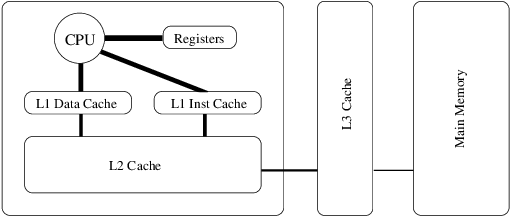
\includegraphics[width=\textwidth]{images/memory_layout.png}}
    \only<2>{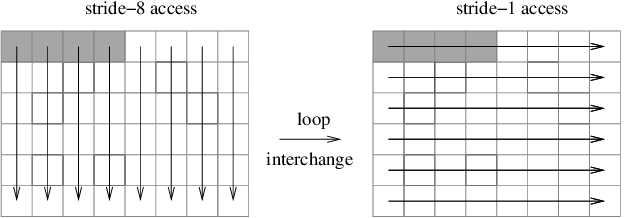
\includegraphics[width=\textwidth]{images/access_patterns.png}}
    \only<3>{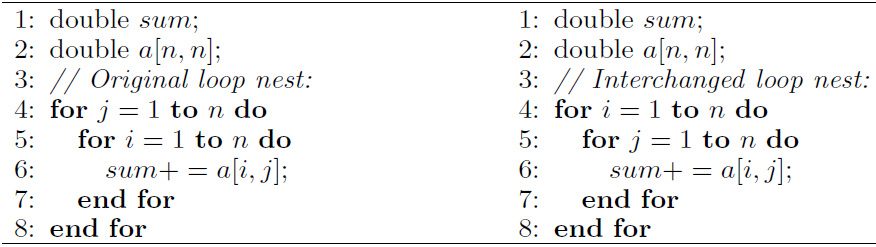
\includegraphics[width=\textwidth]{images/loop_tiling.png}}
\end{figure}
\end{frame}

\begin{frame}{Exercise 1.3}
\begin{itemize}
\item Include the {\tt Eigen/Dense} header.
\item Use the {\tt Eigen::Map} template class to wrap the matrix data and interpret it as {\tt Eigen::MatrixXd}.
\item Compare the execution speed with respect to the previous implementations.
\end{itemize}
\end{frame}

\begin{frame}{Exercise 2}
The program \texttt{integer-list} in the directory \texttt{02-bug} has:

\begin{itemize}
    \item One compile error.
    \item One run-time error.
    \item One memory leak.
    \item A potential memory leak that is not captured by the main.
\end{itemize}
\vfill
Find all the issues and fix them. \\[3mm]

The directory \texttt{02-bug-solution} contains the fixed code,
please don't look at it before trying to solve the exercise by yourself.
\end{frame}

\end{document}
